\scanpage{152}
% archive sheet number: 151
géométrique de $S$, $\xi_i$ son image dans $S_i$, donc
\[
\unsure{\pi_1|\pi}=\pi_1(S,\xi)\xrightarrow{\sim}\varprojlim_i\pi_i\unsure{[|;}\qquad \pi_i=\pi_1(S_i,\xi_i).
\]
Donc un élément (disons) de $\unsure{\mathcal V|\mathscr V}_\ell(\unsure{\mathscr S|\mathcal S})$ \deleted{s'identifie \unsure{essentiellement à un}} est défini par un vectoriel $V_{\unsure{\ell|i}}$ sur $\mathbb Q_\ell$ où $\pi_i$ opère ``continûment'', avec le ``proviso'' que pour un $W_j$ analogue sur $\pi_j$, un ``homomorphisme'' de $V$ dans $W$ est un élément de
\[
\varinjlim_{\substack{k\\(k\geq i,j)}}\operatorname{Hom}_{S_k}(V_i\times_{S_i}S_k,\;W_j\times_{\unsure{\varphi_j|S_j}}S_k)
\]

% vertical emphasis line in left margin
\margin{\rule{0.4pt}{6\baselineskip}}
Supposons maintenant que \inserted{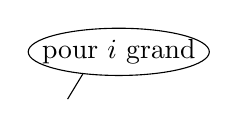
\begin{tikzpicture}[baseline=(n.base)]\node (n) at (0,0) {pour $i$ grand};\draw (0,0) ellipse (1.15 and .3);\draw (-.45,-.27)--(-.65,-.6);\end{tikzpicture}} les \deleted{\unsure{$S_i$}} hom \deleted{$\pi_1(S_j,\unsure{\xi|\xi_j})$} $\pi_j\longrightarrow\pi_i$ aient des images d'indice fini. Cela est le cas si les $S_i$ sont \uline{normaux} \inserted{pour $i$ grand}, et les $\varphi_{ij}:S_j\unsure{\text{---}|\longrightarrow}S_i$ sont dominants et \inserted{définissent des extensions de corps} de type fini.

[on est ramené au cas des \uline{corps}, où on distingue le cas d'une extension \unsure{transcendante}
